\documentclass[11pt,a4paper]{article}

\usepackage[T1]{fontenc}
\usepackage[utf8]{inputenc}
\usepackage{lmodern}
\usepackage[margin=2.4cm]{geometry}
\usepackage{microtype}
\usepackage{graphicx}
\usepackage{booktabs}
\usepackage{array}
\usepackage{amsmath,amssymb}
\usepackage{caption}
\usepackage{float}
\renewcommand{\topfraction}{0.9}\renewcommand{\textfraction}{0.08}\renewcommand{\floatpagefraction}{0.8}
\usepackage{xcolor}
\usepackage[numbers,sort&compress]{natbib}
\usepackage[colorlinks=true,linkcolor=blue!50!black,citecolor=blue!50!black,urlcolor=blue!50!black]{hyperref}

\graphicspath{{../figures/}}
\captionsetup{font=small,labelfont=bf}
\setlength{\parskip}{0.35em}

\newcommand{\Sone}{S1}
\newcommand{\arr}{$\rightarrow$}

\title{\textbf{Session-to-Session Drift in Motor-Imagery Decoding}\\[0.3em]
\large A pre-specified test on BNCI2014-004 (BCI Competition IV 2b)}
\author{\begin{tabular}{cc}
Aruzhan Nurmanova & Sultanbek Myrzakhmet\\
Daniela Gabdullina & Aidar Toktargazin
\end{tabular}\\[0.8em]
\normalsize ROBT613 --- Brain--Computer Interfaces, Midterm Project}
\date{November 2026}

\begin{document}
\maketitle

\begin{abstract}
A brain--computer interface (BCI) is usually calibrated on one day and used on later days. Electrode placement,
impedance, fatigue and learning all change between days, so the EEG features a decoder relies on may shift
(\emph{session-to-session drift}). We tested, with hypotheses and decision rules fixed in advance, whether a
left- vs.\ right-hand motor-imagery decoder trained on an earlier day performs worse on a new day than a decoder
trained on that same day. Using BNCI2014-004 (9 subjects, 5 sessions on different days, 3 bipolar EEG channels),
we built an offline pipeline in MNE-Python restricted to the methods of the BCI Workshop notebooks 00--06:
FIR filtering, EOG regression fitted on a separate eye-movement calibration recording, trial cleaning applied to
training data only, log band-power features and logistic regression. Within- and cross-session decoders were
compared with matched training-set sizes and scored run by run on identical trials. We found \textbf{no measurable
drift in class separation}: median drift cost was $-0.002$ AUC for screening day 1\arr2 ($p=0.55$) and $+0.003$ AUC
for feedback sessions 3\arr4/5 ($p=0.08$). What does drift is the decision threshold: balanced accuracy at the
default threshold dropped slightly but consistently in feedback sessions ($+0.011$, $p=0.014$). Neither
label-free fix (baseline-relative power; per-session z-scoring) reduced the drift cost, and baseline-relative
power made decoding worse. The conclusion held in all six pre-planned sensitivity analyses. We also show that
leave-one-session-out evaluation hides drift, because more training data outweighs day-to-day change.
\end{abstract}

%======================================================================
\section{Introduction}
%======================================================================
A working BCI depends on a chain of choices --- recording, cleaning, segmentation, feature extraction, decoding and
evaluation --- and a weakness at any step can make a system look better or worse than it is. In practice a
motor-imagery (MI) BCI is calibrated once and then used over several days. If the features it relies on move between
days, a decoder trained on an earlier day should do worse on a new day than a decoder trained on that same day. This
\emph{session-to-session drift} is often cited as a reason for frequent recalibration, but it is easy to measure
wrongly: comparisons that give the cross-session decoder more (or less) training data than the within-session decoder,
or that score the two on different trials, confound drift with training-set size and scoring artefacts.

Following the methods of the ROBT613 BCI Workshop notebooks 00--06~\cite{workshop}, our study asks a narrow question and answers it with a controlled comparison: \emph{does left/right separation drop on a
new day, once both decoders get the same amount of training data and are scored on the same trials?}

\paragraph{Disclosed history.} A first version of this study (v1) used MOABB's ready-made epochs, an EOG correction fitted
on task data, no trial cleaning and imprecise band edges; it found no drift for day 1\arr2. The hypotheses below were
written before v1's results and are kept unchanged. What is new in this version is the data preparation (fixed
independently of this question for our second study) and hypothesis H1b, which was added and fixed before it was run
for the first time.

%======================================================================
\section{Hypotheses and decision rules}
%======================================================================
All hypotheses, tests and the significance level were fixed before the analysis (Table~\ref{tab:hyp}, Fig.~\ref{fig:design}).
The \emph{drift cost} of a subject is
\begin{equation}
  \text{drift cost} = \text{AUC}_\text{within} - \text{AUC}_\text{cross},
\end{equation}
where $\text{AUC}_\text{within}$ comes from cross-validation inside the scored session and
$\text{AUC}_\text{cross}$ from a decoder trained on the earlier session, with the same number of training trials.
A positive drift cost means the decoder from the earlier day is worse.

\begin{table}[H]
\centering\small
\caption{Pre-specified hypotheses. All tests are over the 9 subjects, $\alpha=0.05$.}
\label{tab:hyp}
\begin{tabular}{@{}>{\raggedright\arraybackslash}p{2.4cm}>{\raggedright\arraybackslash}p{8.4cm}>{\raggedright\arraybackslash}p{4.4cm}@{}}
\toprule
 & Hypothesis & Test \\
\midrule
\textbf{H1a}\newline(primary) & Trained on session 1, tested on session 2 (both screening, different days): ROC AUC is \emph{lower}
than within-session cross-validation on session 2, with the same number of training trials. & drift cost $>0$; one-sided Wilcoxon signed-rank \\
\textbf{H1b}\newline(secondary, new) & Same inside the feedback paradigm: trained on session 3, tested on sessions 4 and 5 (averaged). & same \\
\textbf{H2}\newline(fixes) & Two label-free fixes reduce the drift cost: \textbf{C} baseline-relative power (log power 3.5--5.5\,s minus
0.5--1.5\,s) and \textbf{D} per-session z-scoring of features (the team's README hypothesis). & drift cost averaged over
both transfers; one-sided Wilcoxon per fix, Holm-corrected; cross-session AUC must not drop significantly \\
\bottomrule
\end{tabular}
\end{table}

\textbf{Secondary metric.} Everywhere we also report balanced accuracy at the default decision threshold. AUC only asks
whether right-hand trials score higher than left-hand trials; if a new day shifts \emph{all} scores together, AUC is
unchanged but accuracy drops. Comparing the two metrics therefore tells us \emph{which kind} of drift is present.

\begin{figure}[!htbp]
\centering
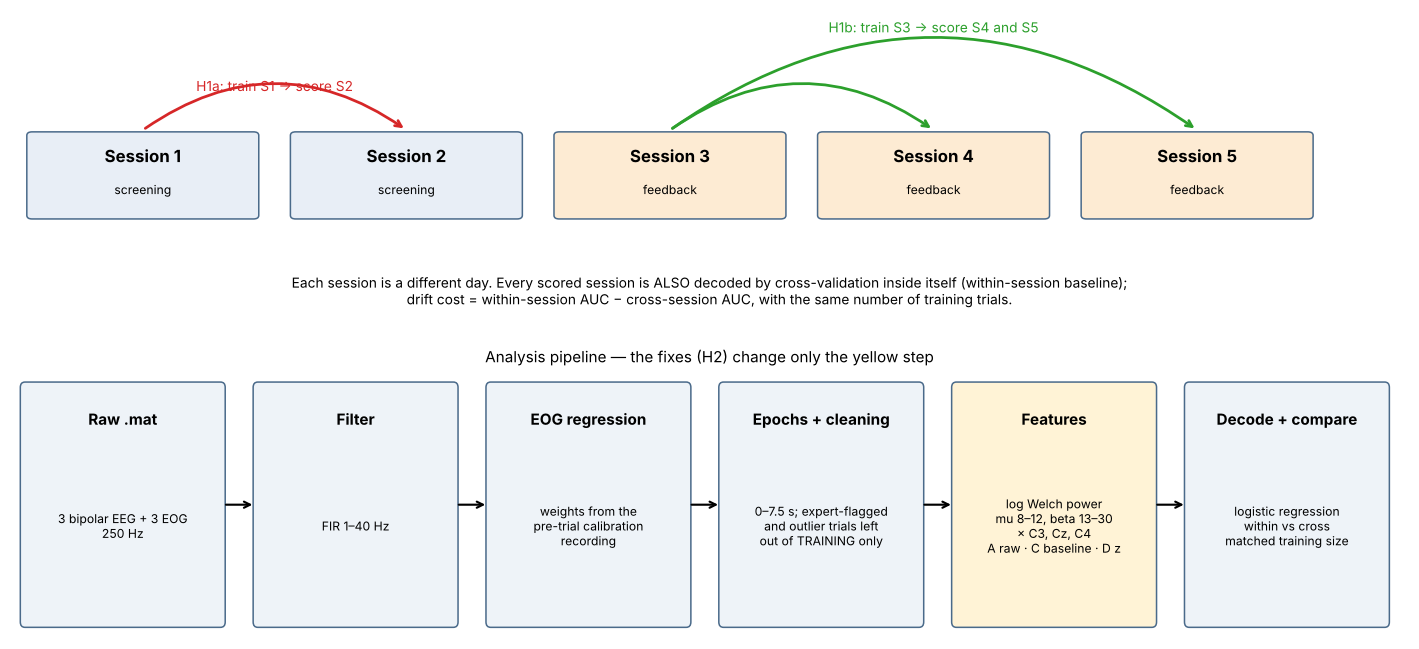
\includegraphics[width=\linewidth]{study_design.png}
\caption{Study design. Top: the two transfers (H1a: train S1, score S2; H1b: train S3, score S4 and S5). Every scored
session is also decoded by cross-validation inside itself. Bottom: the analysis pipeline; the fixes of H2 change only the
feature step (yellow).}
\label{fig:design}
\end{figure}

%======================================================================
\section{Dataset}
%======================================================================
BNCI2014-004 is data set 2b of BCI Competition IV, recorded in Graz~\cite{leeb2008}. Nine subjects
(4 female, 5 male, 20--32 years) performed cued left- vs.\ right-hand motor imagery in five sessions on different days.
Sessions 1--2 are \emph{screening} sessions without feedback (120--160 trials, runs of 20 trials); sessions 3--5 provide
online \emph{smiley feedback} (120--160 trials, runs of 40 trials). The EEG consists of three bipolar channels around C3, Cz
and C4 (electrodes about 2.5\,cm apart) plus three EOG channels, sampled at 250\,Hz.

We read the original competition \texttt{.mat} files ourselves (MOABB~\cite{jayaram2018} was used only to download them),
which keeps every field the authors provide: signals, trial onsets, labels, expert artifact flags, age and gender.

\paragraph{Data audit.} Sampling rate was 250\,Hz in every session, and left and right trials were balanced in every
session. Most sessions contain 120 (screening) or 160 (feedback) trials; four sessions differ and we used what the files
contain (6{,}520 trials in total). The dataset authors flagged 1{,}253 trials (19.2\,\%) as artifacts. The most important
audit finding was the time before the first trial: in most sessions it is about 3.6\,min long. This is the recording of
deliberate eye movements and blinks that the dataset description says precedes each session; we use it to fit the EOG
correction (Section~\ref{sec:prep}). Figure~\ref{fig:audit} summarises the audit.

\begin{figure}[!htbp]
\centering
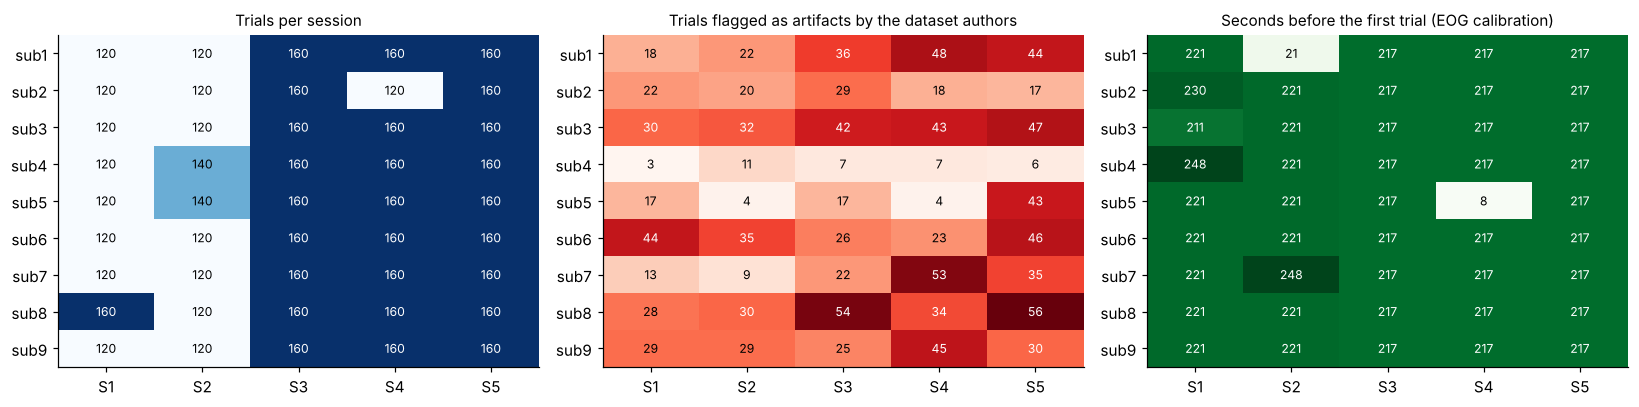
\includegraphics[width=\linewidth]{data_audit.png}
\caption{Data audit per subject and session: trial counts (left), trials flagged as artifacts by the dataset authors
(middle), and seconds before the first trial, i.e.\ the eye-movement calibration recording (right).}
\label{fig:audit}
\end{figure}

\paragraph{Where the signal comes from.} C3 and C4 lie over the left and right hand area of primary motor cortex~\cite{mayka2006}. Each hand
is controlled by the contralateral hemisphere, so imagining the right hand should reduce mu/beta power at C3 and imagining
the left hand should reduce it at C4 (event-related desynchronisation, ERD~\cite{pfurtscheller1999}). Because each channel
is a closely spaced bipolar pair, it mainly reflects cortex directly underneath. With three bipolar channels we cannot
localise sources; Fig.~\ref{fig:sites} shows what each channel sits over, not a source estimate.

\begin{figure}[!htbp]
\centering
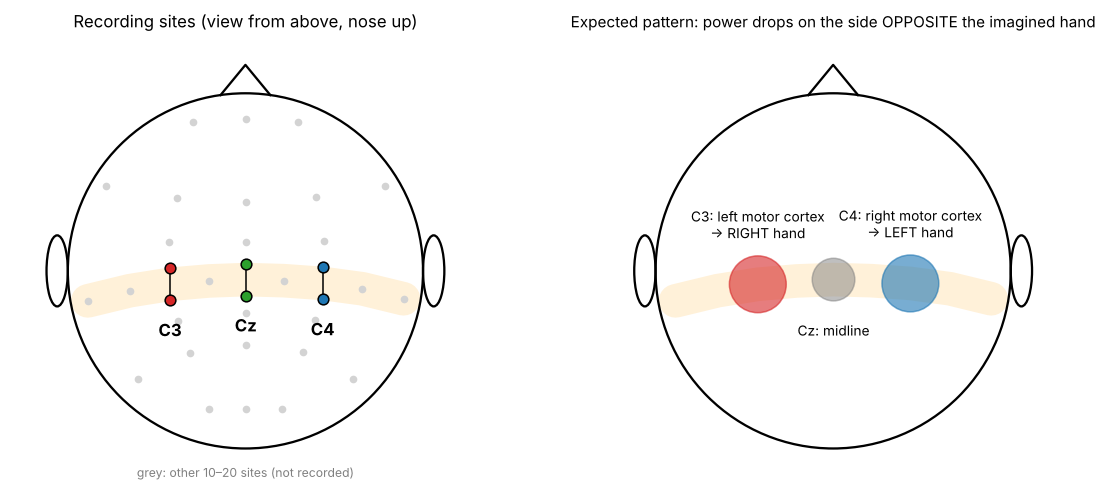
\includegraphics[width=0.85\linewidth]{recording_sites.png}
\caption{Recording sites (left) and the expected contralateral pattern (right): power drops on the side opposite the
imagined hand.}
\label{fig:sites}
\end{figure}

%======================================================================
\section{Preprocessing}\label{sec:prep}
%======================================================================
The same steps were applied to every session and to both arms of every comparison. No step uses class labels.
\begin{enumerate}\itemsep0.2em
  \item \textbf{Units and MNE object.} The files store data in $\mu$V; we converted to volts and built an MNE
        \texttt{RawArray}~\cite{gramfort2013}. The channels are already bipolar, so no re-referencing was applied.
  \item \textbf{FIR band-pass 1--40\,Hz} (zero-phase, \texttt{firwin}) on the continuous signal. This removes slow drift
        and keeps everything up to the highest feature band edge (30\,Hz). The amplifier had already notched 50\,Hz line noise.
  \item \textbf{EOG regression.} We estimated how much each EOG channel leaks into each EEG channel from the
        \emph{pre-trial calibration recording}, in which the subject moved the eyes on purpose, and subtracted that leak
        from the whole session (MNE \texttt{EOGRegression}). A separate recording is cleaner than fitting on task data
        and uses no labels. 43 of 45 sessions had at least 60\,s of calibration; the remaining two fell back to fitting on
        the whole session (also label-free).
  \item \textbf{Epochs} from 0 to 7.5\,s after trial start. The cue appears at about 3\,s in both paradigms; features are taken
        from 3.5--5.5\,s and the baseline for fix C from 0.5--1.5\,s (Fig.~\ref{fig:timeline}).
  \item \textbf{Trial cleaning, training data only.} A trial is left out of training if the dataset authors flagged it, or if
        its EEG log-variance is more than 5 robust SDs (median $\pm\,5\times1.4826\times$MAD) from the session median on any
        channel. This applies to the training session in cross-session tests \emph{and} to the training folds of within-session
        cross-validation. \textbf{Scored trials are never removed}: an online BCI must classify every trial, and both
        comparisons are scored on exactly the same trials. Over all sessions, 1{,}272 of 6{,}520 trials (19.5\,\%) would be
        left out of training: 1{,}253 expert-flagged and 19 additional variance outliers.
\end{enumerate}

\begin{figure}[!htbp]
\centering
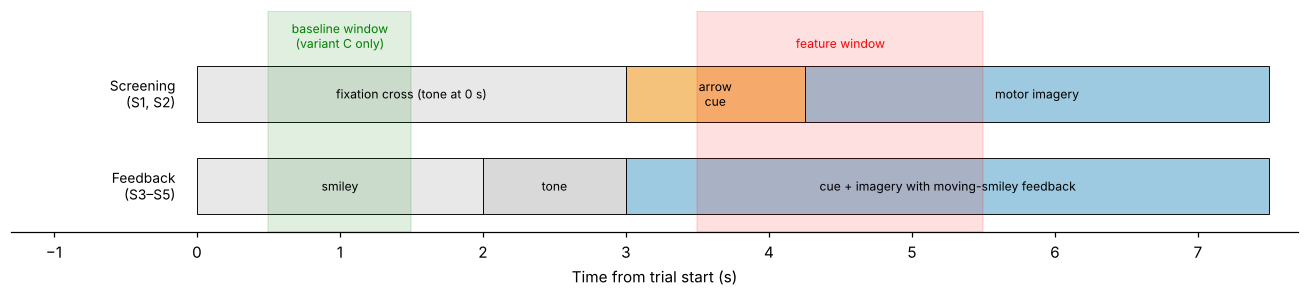
\includegraphics[width=0.9\linewidth]{trial_timeline.png}
\caption{Trial timeline of the two paradigms with the baseline window (green, used only by fix C) and the feature window (red).}
\label{fig:timeline}
\end{figure}

\begin{figure}[!htbp]
\centering
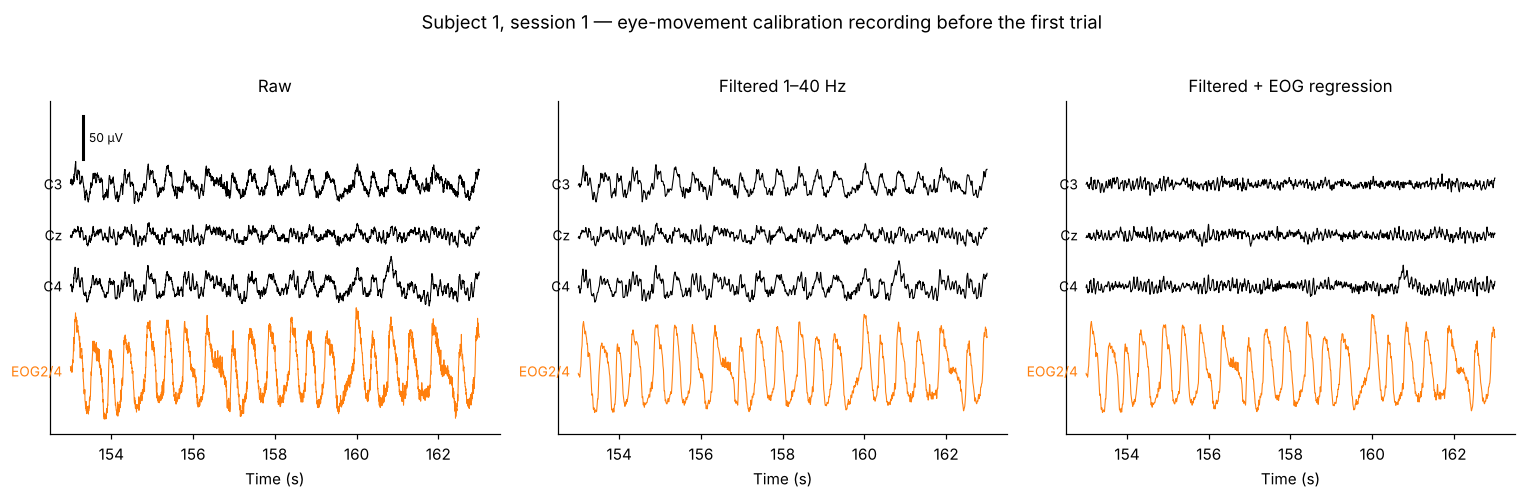
\includegraphics[width=\linewidth]{eog_regression.png}
\caption{EOG regression on the calibration recording of subject 1, session 1: raw signal, after the 1--40\,Hz filter, and after
regression. Eye movements (orange, EOG2 scaled by 1/4) leak into the EEG channels; regression removes the leak.}
\label{fig:eog}
\end{figure}

\begin{figure}[!htbp]
\centering
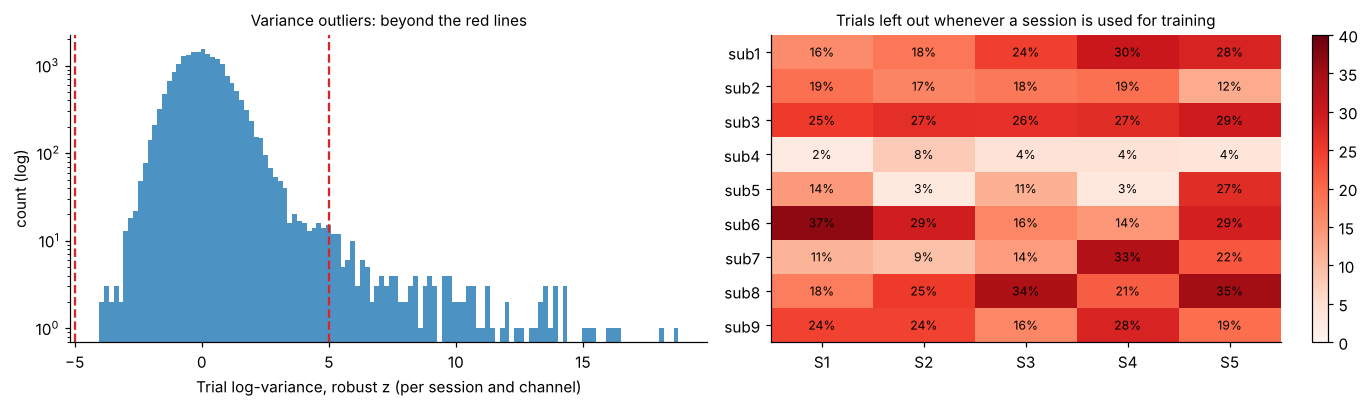
\includegraphics[width=\linewidth]{trial_cleaning.png}
\caption{Trial cleaning. Left: distribution of trial log-variance in robust-z units; trials beyond the red lines are outliers.
Right: percentage of trials left out whenever a session is used for training.}
\label{fig:cleaning}
\end{figure}

%======================================================================
\section{Is the expected brain response present?}
%======================================================================
Before decoding anything, we checked for the physiological response. ERD was computed as the percentage change of band power
relative to the pre-cue period (0.5--2.5\,s), averaging over trials first~\cite{pfurtscheller1999}. Band power was taken as the
squared Hilbert envelope of the band-passed signal.

After the cue, power drops more at C3 for right-hand imagery and more at C4 for left-hand imagery, in both mu and beta bands and
in both paradigms (Fig.~\ref{fig:erd}). The time--frequency map of signed $r^2$ between band power and class confirms the
contralateral pattern and shows that the feature window and bands sit where the classes separate (Fig.~\ref{fig:tf}).

\begin{figure}[!htbp]
\centering
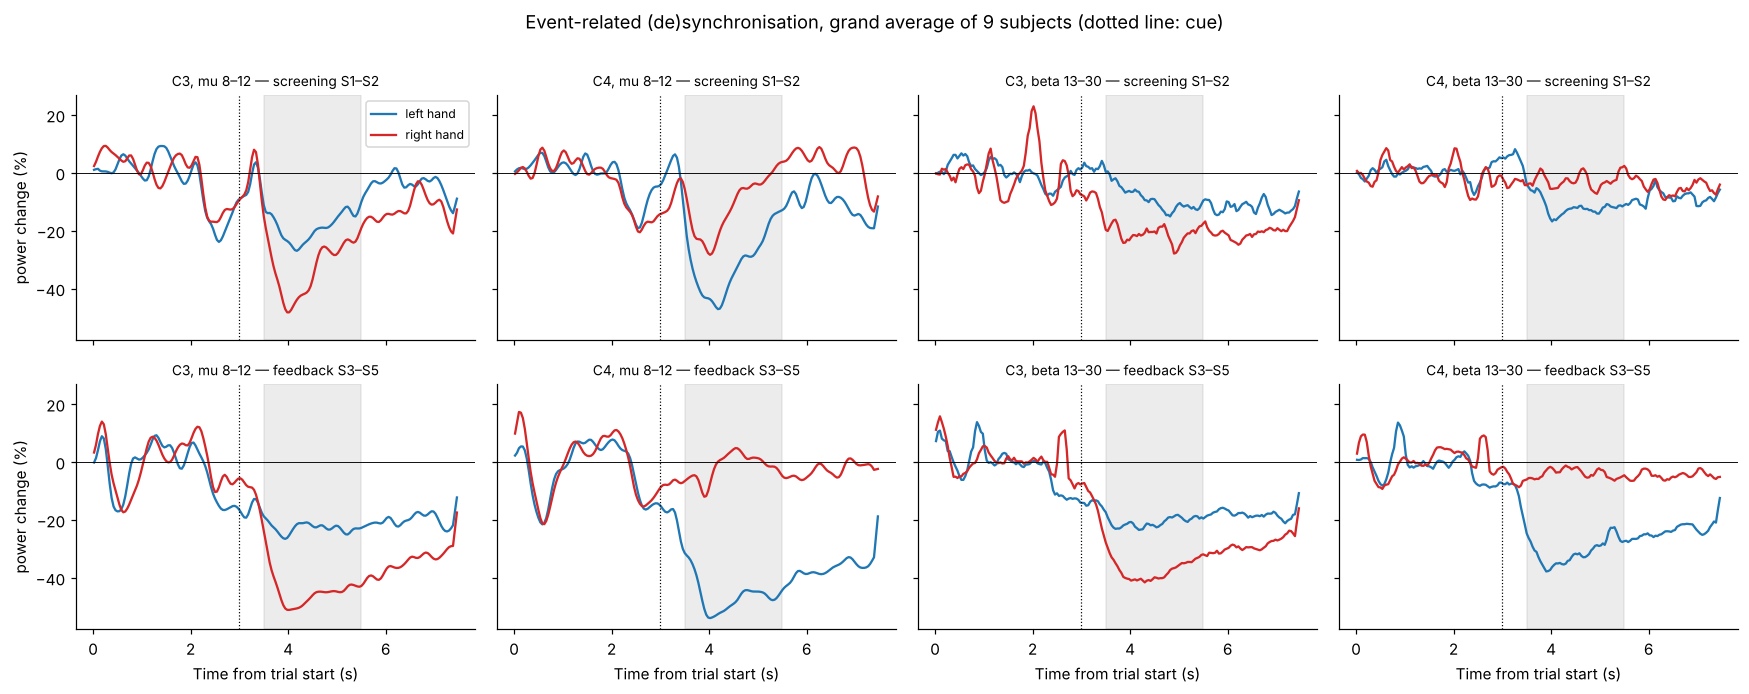
\includegraphics[width=\linewidth]{erd.png}
\caption{Event-related (de)synchronisation, grand average of 9 subjects, for screening (top) and feedback sessions (bottom).
Dotted line: cue; grey: feature window.}
\label{fig:erd}
\end{figure}

\begin{figure}[!htbp]
\centering
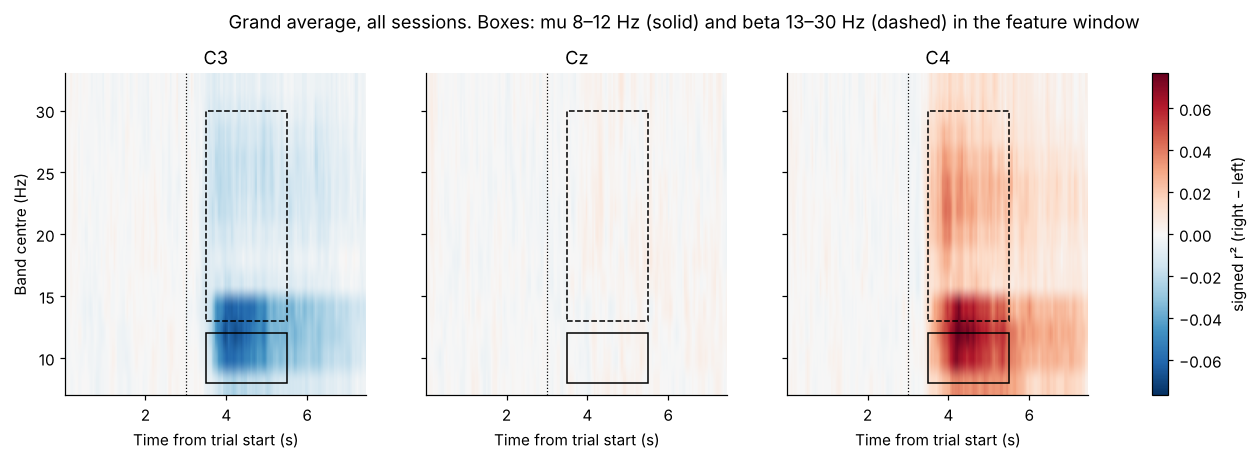
\includegraphics[width=\linewidth]{time_frequency.png}
\caption{Signed $r^2$ between band power and class (right $=+1$), all sessions, grand average. Blue at C3 and red at C4 is the
expected contralateral ERD. Boxes: mu 8--12\,Hz (solid) and beta 13--30\,Hz (dashed) in the feature window.}
\label{fig:tf}
\end{figure}

%======================================================================
\section{Features, decoder and evaluation}
%======================================================================
\paragraph{Features.} For each trial we computed the Welch PSD (1\,Hz resolution) in the 3.5--5.5\,s window, averaged the 1-Hz bins
8--12\,Hz (mu) and 13--30\,Hz (beta) at C3, Cz and C4, and took the natural log, giving 6 features. Three variants were compared:
\begin{itemize}\itemsep0.1em
  \item \textbf{A} raw log power --- the standard pipeline;
  \item \textbf{C} baseline-relative --- each trial's log power in 3.5--5.5\,s minus its own log power in 0.5--1.5\,s, which cancels
        a day-specific overall power level;
  \item \textbf{D} session z-scored --- each feature standardised with the mean and SD of all trials of its own session (no labels).
        D needs unlabelled data from the new day; sensitivity analysis (c) uses only the new day's first run for this and scores
        the remaining runs, which is the realistic online version.
\end{itemize}

\paragraph{Decoder.} A standard scaler followed by L2-regularised logistic regression ($C=1$), refitted inside every fold
(scikit-learn~\cite{pedregosa2011}).

\paragraph{Evaluation without leakage.} For a training session $a$ and a scored session $b$:
\begin{itemize}\itemsep0.1em
  \item \textbf{Within-session:} leave-one-run-out cross-validation inside $b$. Training folds use only cleaned trials; every
        trial of the held-out run is scored. A run is never on both sides (checked by assertion).
  \item \textbf{Cross-session:} fit on the cleaned trials of $a$; score every trial of $b$.
  \item \textbf{Same scoring on both sides:} AUC is computed run by run on exactly the same trials for both decoders and then
        averaged over runs.
  \item \textbf{Matched training size:} both decoders get the same number of training trials (the smaller of the two), drawn
        class-stratified at random 20 times; results are averaged. For subject 1 this is 79 trials for S1\arr S2 and 81/83 for
        S3\arr S4/S5.
\end{itemize}

\paragraph{Validation checks.} (V1) A run is never in both training and test sets. (V2) With training labels shuffled
(20 times per subject and transfer), mean AUC was 0.502 on the within side and 0.501 on the cross side, i.e.\ at chance
(Fig.~\ref{fig:v2}); a wide spread is expected because a decoder trained on noise points in a random direction. (V3) The
cross-session decoder is above chance (one-sided Mann--Whitney $p<0.05$) in 7 of 9 subjects for each transfer.

\begin{figure}[!htbp]
\centering
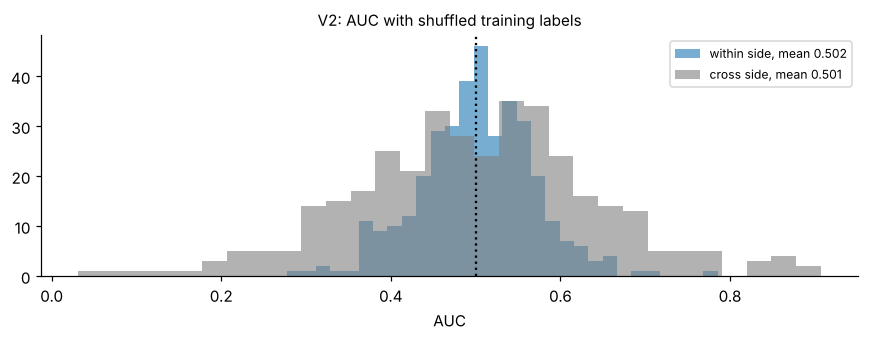
\includegraphics[width=0.62\linewidth]{v2_shuffle.png}
\caption{V2: AUC with shuffled training labels stays centred at 0.5 on both sides.}
\label{fig:v2}
\end{figure}

%======================================================================
\section{Results}
%======================================================================
\subsection{Drift visible before decoding}
Without labels or a decoder, the overall mu power level clearly moves between days for most subjects (Fig.~\ref{fig:drift},
left); the baseline-relative variant moves less. Decoded on its own, each day reaches a median within-session AUC of
0.731 (S1), 0.649 (S2), 0.895 (S3), 0.843 (S4) and 0.894 (S5): subjects decode much better once feedback starts.

The discriminative pattern, however, is stable. The grand-average class contrast on the head is blue at C3 and red at C4 every
day (Fig.~\ref{fig:head}), and decoders fitted separately on each day rely on the same features: mu and beta at C3 negative,
at C4 positive, with cosine similarity between days of 0.63--0.84 (Fig.~\ref{fig:weights}).

\begin{figure}[!htbp]
\centering
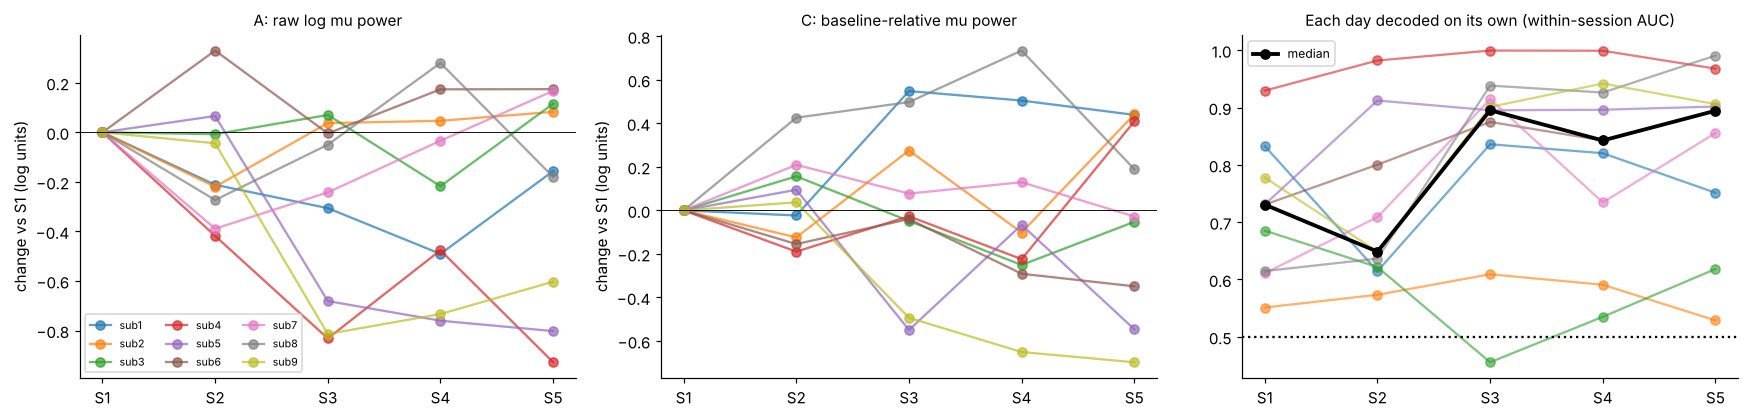
\includegraphics[width=\linewidth]{drift_before_decoding.png}
\caption{Left and middle: change of mean log mu power (C3, C4) relative to S1, one line per subject, for raw (A) and
baseline-relative (C) features. Right: within-session AUC per day (black: median).}
\label{fig:drift}
\end{figure}

\begin{figure}[!htbp]
\centering
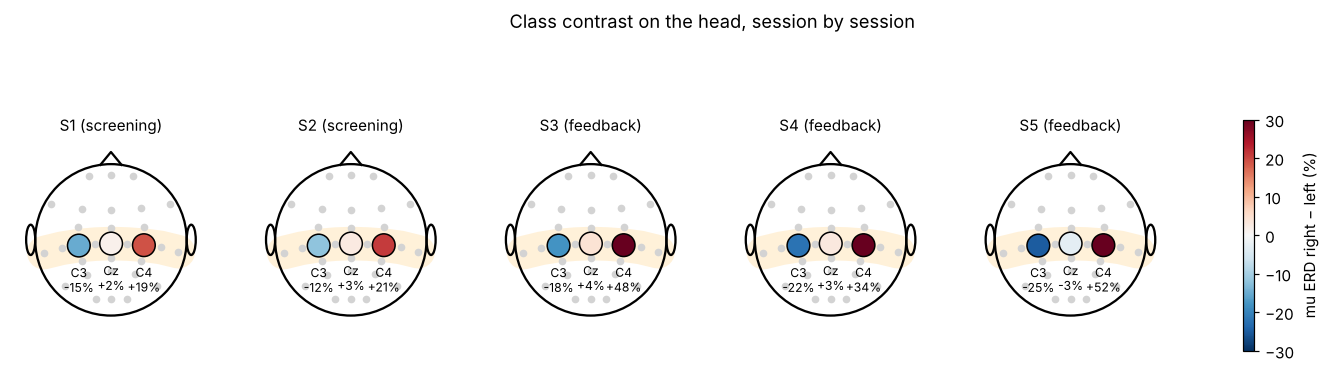
\includegraphics[width=\linewidth]{head_contrast.png}
\caption{Mu ERD contrast (right minus left imagery) in the feature window, grand average, session by session.}
\label{fig:head}
\end{figure}

\begin{figure}[!htbp]
\centering
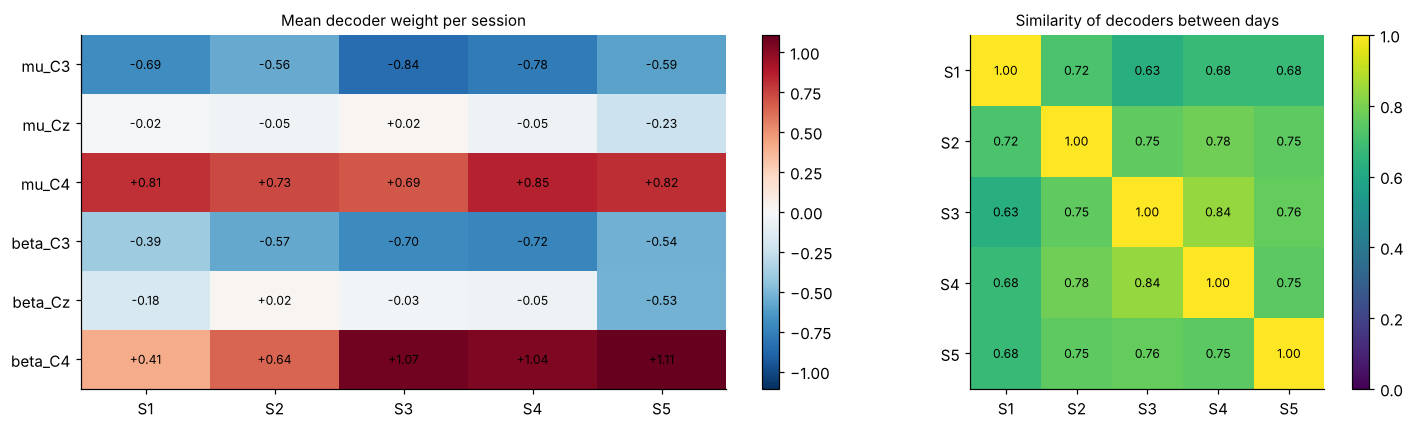
\includegraphics[width=\linewidth]{decoder_weights.png}
\caption{Left: mean decoder weight per session (positive $\rightarrow$ ``right hand''). Right: cosine similarity between the weight
vectors of every pair of days, averaged over subjects.}
\label{fig:weights}
\end{figure}

\subsection{H1: does performance drop on a new day?}
Table~\ref{tab:h1} and Fig.~\ref{fig:h1} give the primary result. With matched training size and identical scored trials, the
decoder trained on an earlier day separated left from right hand on the new day as well as a decoder trained on that same day.
\textbf{H1a is not supported} (median drift cost $-0.002$ AUC, positive in 4/9 subjects, $p=0.545$), and \textbf{H1b is not
supported} ($+0.003$, 6/9, $p=0.082$).

The secondary metric tells a different story for feedback sessions: balanced accuracy at the default threshold drops slightly
but consistently ($+0.011$, $p=0.014$). AUC ignores where the threshold sits; accuracy does not. On a new day the whole score
distribution shifts a little while the left/right ordering stays.

\begin{table}[H]
\centering\small
\caption{H1 results (variant A). Medians over 9 subjects; one-sided Wilcoxon signed-rank tests.}
\label{tab:h1}
\begin{tabular}{@{}lcccccccc@{}}
\toprule
 & \multicolumn{2}{c}{Median AUC} & \multicolumn{3}{c}{Drift cost (AUC)} & & \multicolumn{2}{c}{Bal.\ accuracy drift} \\
\cmidrule(lr){2-3}\cmidrule(lr){4-6}\cmidrule(lr){8-9}
Transfer & within & cross & median & positive & $p$ & & median & $p$ \\
\midrule
H1a: S1\arr S2      & 0.677 & 0.656 & $-0.002$ & 4/9 & 0.545 & & $+0.010$ & 0.248 \\
H1b: S3\arr S4/S5   & 0.872 & 0.869 & $+0.003$ & 6/9 & 0.082 & & $+0.011$ & \textbf{0.014} \\
\bottomrule
\end{tabular}
\end{table}

\begin{table}[H]
\centering\small
\caption{Per-subject AUC (variant A, matched training size).}
\label{tab:subj}
\begin{tabular}{@{}ccccccc@{}}
\toprule
 & \multicolumn{3}{c}{S1\arr S2} & \multicolumn{3}{c}{S3\arr S4/S5} \\
\cmidrule(lr){2-4}\cmidrule(lr){5-7}
Subject & within & cross & drift & within & cross & drift \\
\midrule
1 & 0.631 & 0.656 & $-0.025$ & 0.796 & 0.773 & $+0.023$ \\
2 & 0.593 & 0.633 & $-0.040$ & 0.558 & 0.557 & $+0.001$ \\
3 & 0.628 & 0.628 & $\phantom{+}0.000$ & 0.581 & 0.513 & $+0.068$ \\
4 & 0.986 & 0.988 & $-0.002$ & 0.990 & 0.991 & $-0.001$ \\
5 & 0.920 & 0.921 & $-0.002$ & 0.899 & 0.888 & $+0.011$ \\
6 & 0.803 & 0.784 & $+0.020$ & 0.872 & 0.869 & $+0.004$ \\
7 & 0.713 & 0.557 & $+0.156$ & 0.817 & 0.820 & $-0.003$ \\
8 & 0.655 & 0.581 & $+0.074$ & 0.958 & 0.955 & $+0.003$ \\
9 & 0.677 & 0.732 & $-0.055$ & 0.925 & 0.929 & $-0.005$ \\
\bottomrule
\end{tabular}
\end{table}

\begin{figure}[!htbp]
\centering
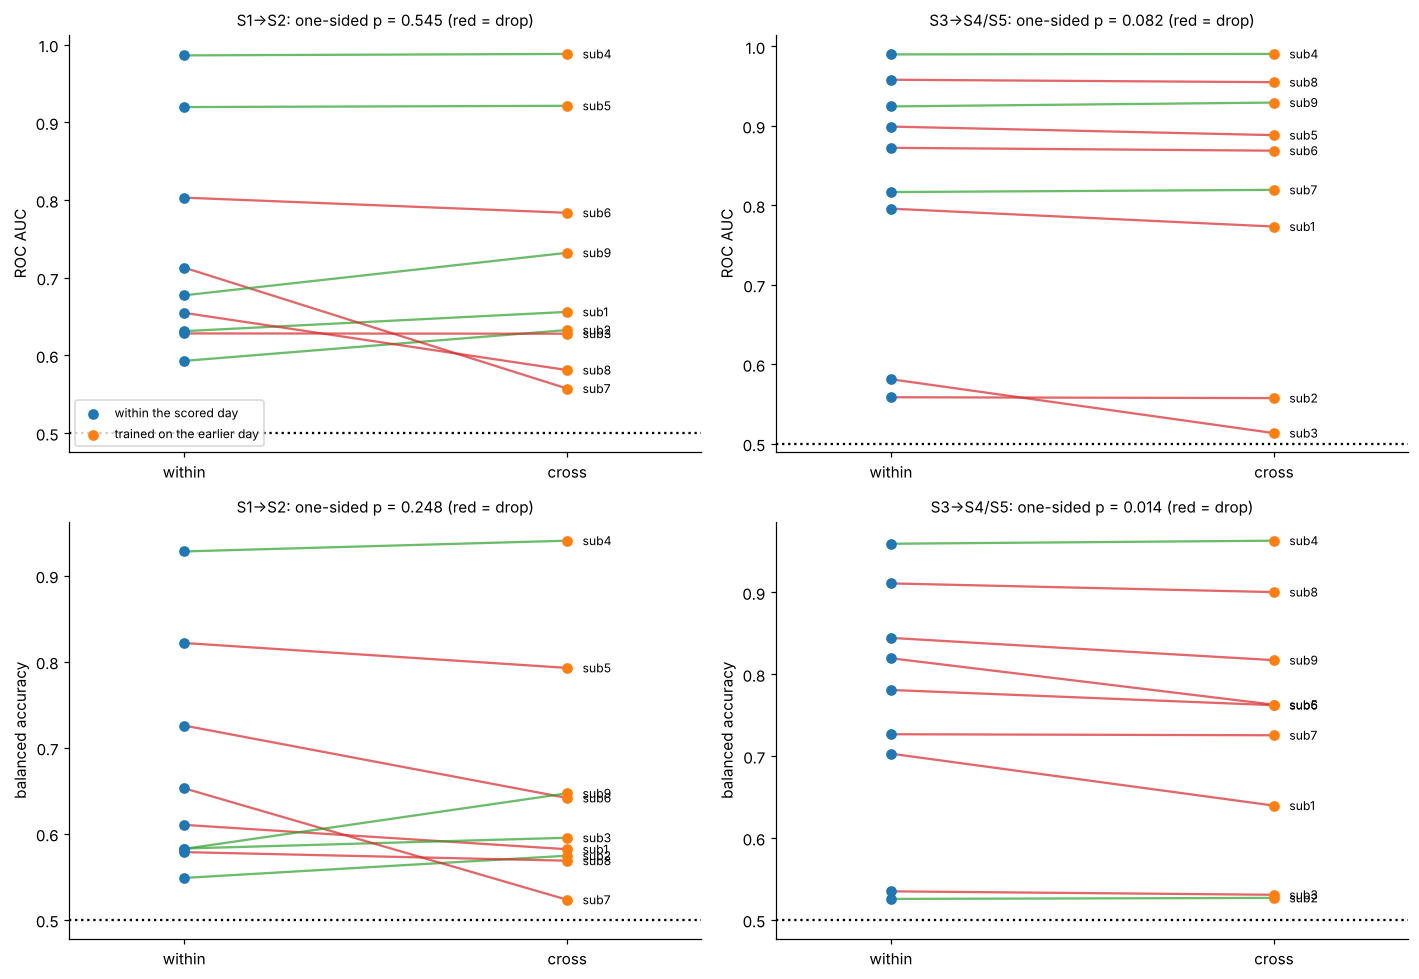
\includegraphics[width=0.92\linewidth]{h1_per_subject.png}
\caption{Within (blue) vs.\ cross-session (orange) performance per subject; red lines are drops. Top: ROC AUC.
Bottom: balanced accuracy at the default threshold.}
\label{fig:h1}
\end{figure}

\begin{figure}[!htbp]
\centering
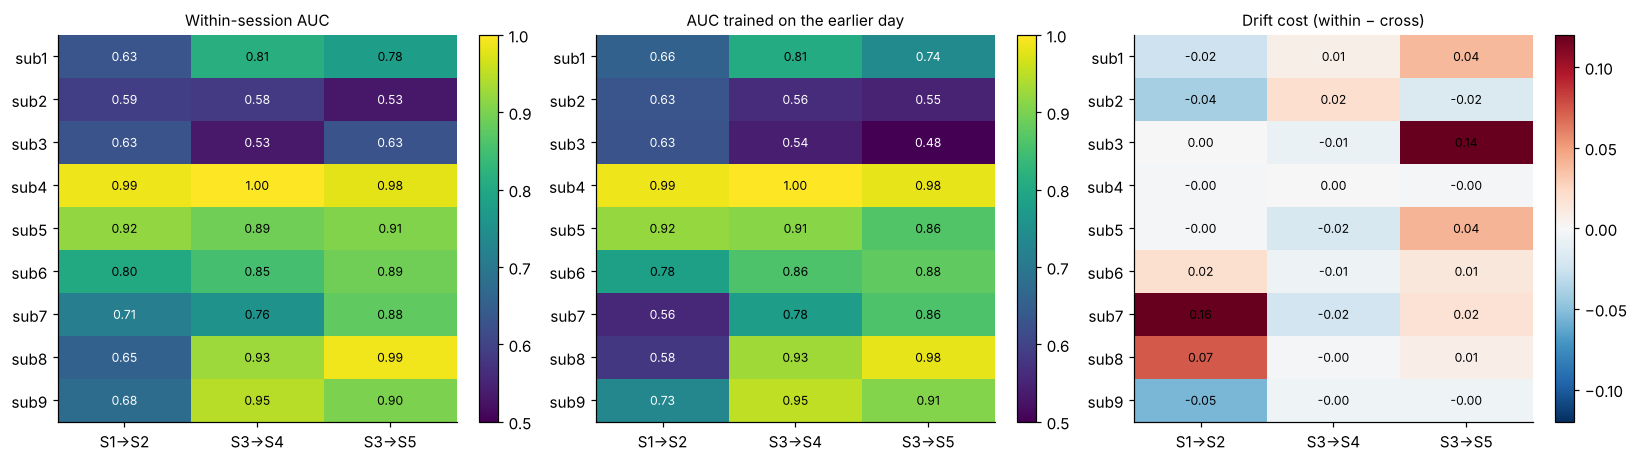
\includegraphics[width=\linewidth]{h1_heatmaps.png}
\caption{Every subject and every scored day: within-session AUC, AUC of the decoder trained on the earlier day, and drift cost.}
\label{fig:heat}
\end{figure}

\paragraph{One subject, one decision line, three days.} To make the mechanism visible we chose one subject by a fixed rule:
among subjects decoded well on S3 (within-session AUC $\ge0.8$), the one whose mean mu power moved most between S3 and S4/S5
(no decoder involved). This is subject 7 (mean shift 0.31 log units). A 2-feature decoder fitted on S3 only and kept fixed
shows the point clouds moving together across days while left and right keep their relative positions
(Fig.~\ref{fig:sub7}; illustration only --- the real decoder uses all six features).

\begin{figure}[!htbp]
\centering
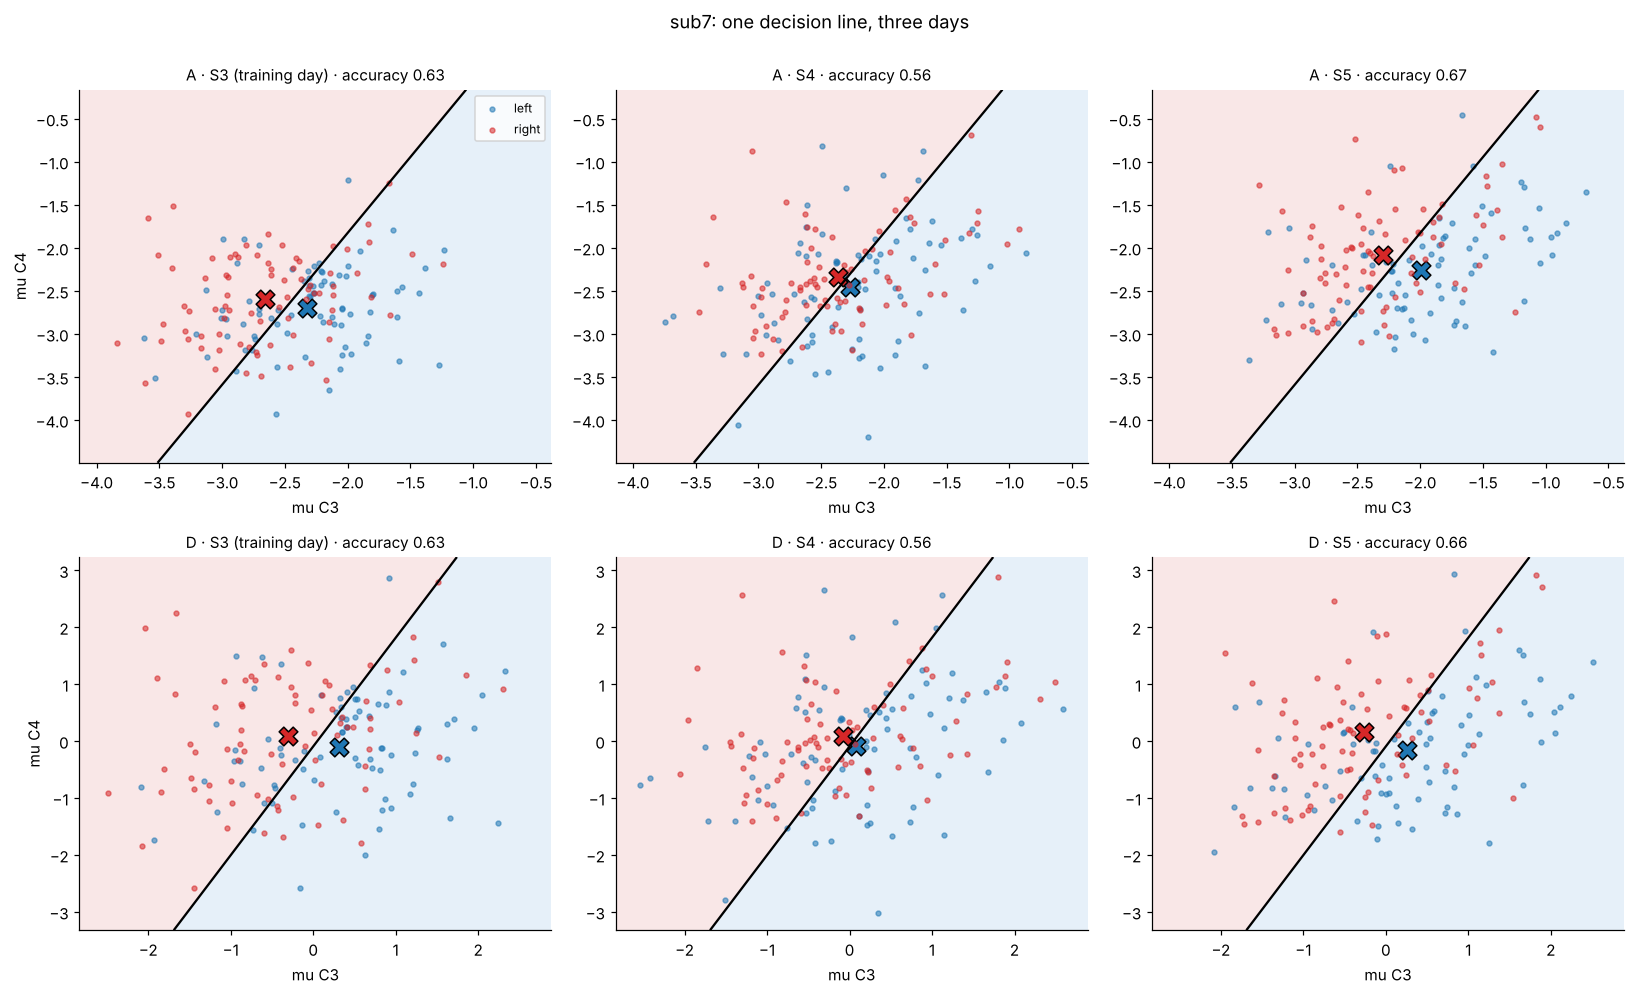
\includegraphics[width=0.95\linewidth]{feature_space_sub7.png}
\caption{Subject 7, trials in the plane of log mu power at C3 (x) and C4 (y), one panel per day. The black line is fitted on S3
only. Top: raw features (A); bottom: session z-scored (D). Titles give the accuracy of the fixed line.}
\label{fig:sub7}
\end{figure}

\subsection{H2: do the fixes reduce the drift cost?}
Neither fix is supported (Table~\ref{tab:h2}, Fig.~\ref{fig:h2}) --- as expected when there is no AUC drift to remove.
Fix C (baseline-relative power) made decoding clearly worse: cross-session AUC fell by 0.066 ($p=0.004$) and within-session AUC
by 0.106. A 1-s single-trial baseline adds noise, and in feedback sessions this window falls on a rising and falling mu
transition. Fix D (session z-scoring) changed nothing in AUC. Because z-scoring is one shift-and-scale per session and the
decoder standardises features anyway, within-session results for D equal those for A by construction; any effect of D can
only appear in cross-session AUC, and none did.

\begin{table}[H]
\centering\small
\caption{H2 results. Drift cost averaged over both transfers; medians over 9 subjects. Reduction $=$ drift(A) $-$ drift(fix).}
\label{tab:h2}
\begin{tabular}{@{}lccccccc@{}}
\toprule
Fix & $\Delta$ within & drift A & drift fix & reduction & Holm $p$ & $\Delta$ cross ($p$) & Supported \\
\midrule
C: baseline-relative & $-0.106$ & 0.005 & 0.003 & $-0.003$ & 0.91 & $-0.066$ (0.004) & no \\
D: session z-scored  & $\phantom{+}0.000$ & 0.005 & 0.010 & $+0.000$ & 0.91 & $+0.000$ (0.91) & no \\
\bottomrule
\end{tabular}
\end{table}

\begin{figure}[!htbp]
\centering
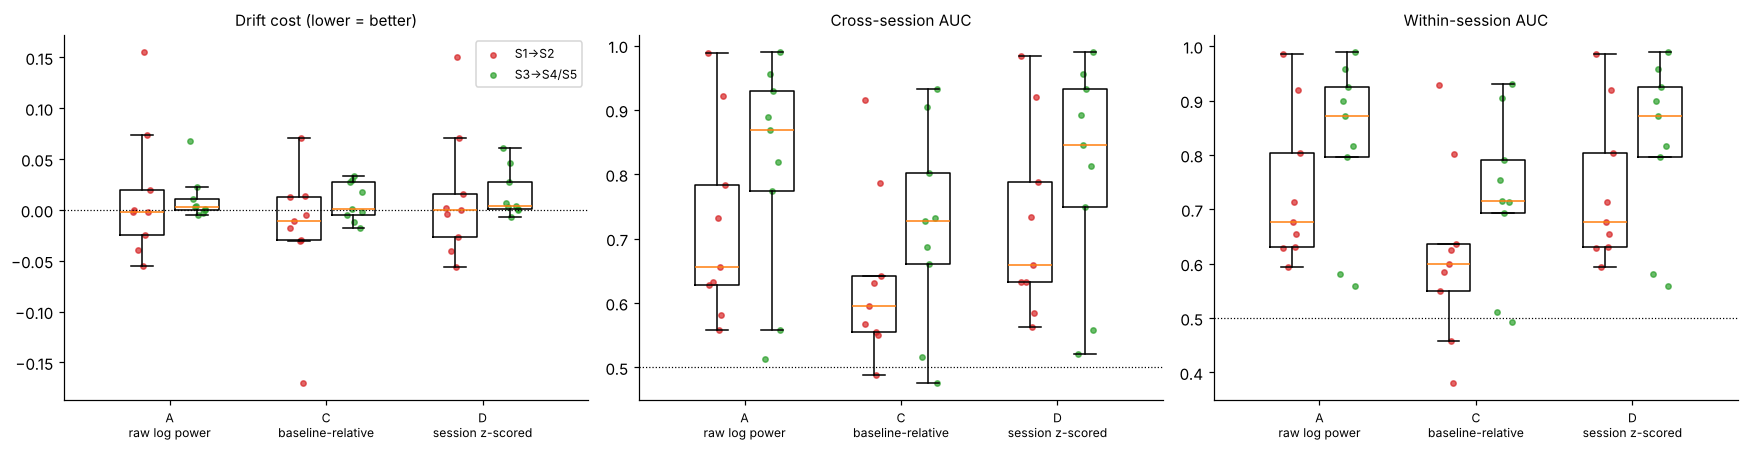
\includegraphics[width=\linewidth]{h2_fixes.png}
\caption{Drift cost, cross-session AUC and within-session AUC for variants A, C and D (red: S1\arr S2; green: S3\arr S4/S5).}
\label{fig:h2}
\end{figure}

\subsection{Why the first notebook found no drift for the wrong reason}
Training size dominates. For the same scored day (S2), median AUC was 0.677 within S2 (matched size), 0.656 trained on S1
(matched), 0.670 trained on all of S1, and 0.697 trained MOABB-style on all four other sessions (median 468 training trials;
Fig.~\ref{fig:size}). Leave-one-session-out training uses days \emph{after} the scored one and beats training on the scored day
itself in 7 of 9 subjects (median $+0.016$ AUC), because more data outweighs any day-to-day change. Such an evaluation cannot
test drift; only matched-size, past-only comparisons can.

\begin{figure}[!htbp]
\centering
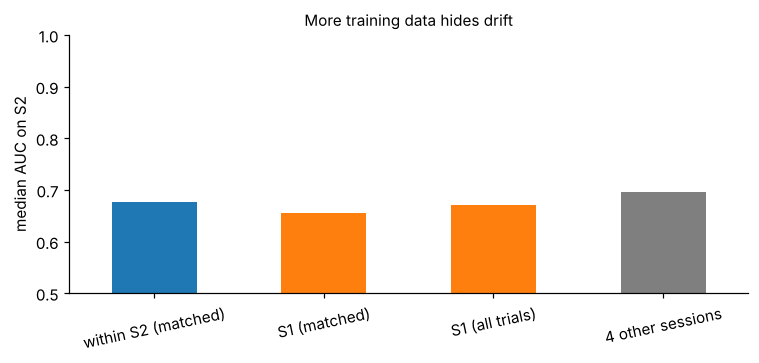
\includegraphics[width=0.55\linewidth]{training_size.png}
\caption{Median AUC on S2 for different training sets: more training data hides drift.}
\label{fig:size}
\end{figure}

\subsection{Sensitivity analyses}
Six analyses were planned in advance (Table~\ref{tab:sens}, Fig.~\ref{fig:sens}). In none of them does H1a or H1b reach
significance, and fix D never reduces the drift cost.

\begin{table}[H]
\centering\small
\caption{Sensitivity analyses: median drift cost (AUC) and one-sided $p$-values.}
\label{tab:sens}
\begin{tabular}{@{}lcccccc@{}}
\toprule
Condition & H1a drift & $p$ & H1b drift & $p$ & D reduction & $p$ \\
\midrule
Main analysis                                   & $-0.002$ & 0.545 & $+0.003$ & 0.082 & $+0.000$ & 0.590 \\
(a) no trial cleaning                           & $+0.003$ & 0.213 & $+0.002$ & 0.213 & $-0.001$ & 0.787 \\
(b) no EOG regression                           & $-0.001$ & 0.590 & $+0.005$ & 0.082 & $-0.002$ & 0.898 \\
(c) new day z-scored from first run only        & $-0.002$ & 0.500 & $+0.009$ & 0.064 & $-0.004$ & 0.787 \\
(d) unmatched training size                     & $-0.001$ & 0.590 & $+0.001$ & 0.180 & $-0.000$ & 0.633 \\
(f) pooled out-of-fold AUC (v1 method)          & $-0.011$ & 0.674 & $+0.002$ & 0.455 & $+0.001$ & 0.590 \\
\bottomrule
\end{tabular}
\par\smallskip\raggedright\footnotesize
(e) Leave-one-session-out training (scored on S2, S4, S5): median within $-$ LOSO $=-0.016$; within wins in only 2/9 subjects.
\end{table}

\begin{figure}[!htbp]
\centering
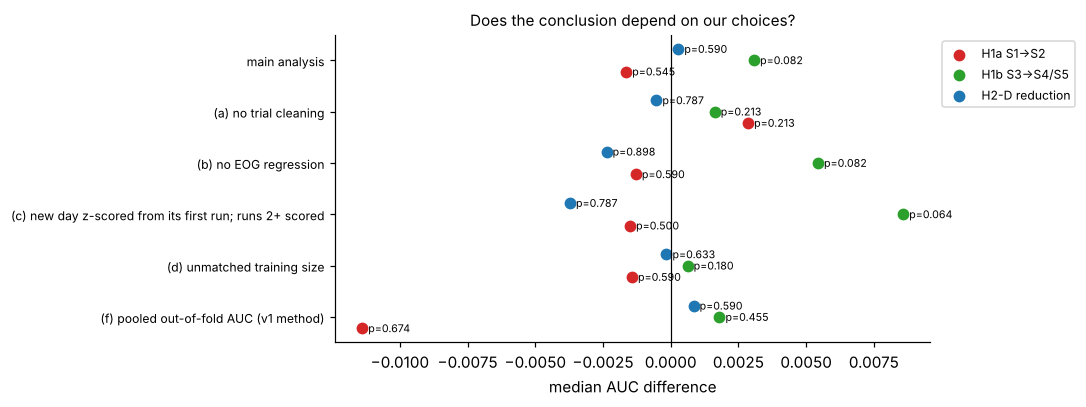
\includegraphics[width=0.85\linewidth]{sensitivity.png}
\caption{Does the conclusion depend on our choices? Median AUC differences with one-sided $p$-values per condition.}
\label{fig:sens}
\end{figure}

%======================================================================
\section{Discussion}
%======================================================================
\paragraph{Answer.} There is no measurable drift in class separation in BNCI2014-004. A decoder trained on an earlier day
separates left from right hand on a new day as well as one trained on that same day, once both have the same amount of training
data. This holds for both transfers and in all six sensitivity analyses.

\paragraph{What does drift.} The decision threshold drifts a little. In feedback sessions balanced accuracy drops slightly but
consistently while AUC does not, which means the score distribution of the new day is shifted as a whole while the ordering of
trials is preserved. This matches the label-free views: the overall mu power level moves between days, while the class contrast
on the head and the decoder weights stay similar. The practical implication is that a new day may need its bias re-estimated,
not the whole decoder.

\paragraph{Why no drift, physiologically.} Subjects improve with feedback: within-session AUC rises from 0.65--0.73 in screening
to 0.84--0.90 in feedback sessions. The contralateral mu pattern becomes stronger rather than weaker, so a decoder from an earlier
day still points in the right direction.

\paragraph{Fixes.} The fixes could not reduce a drift that is not there. Fix C is actively harmful in this dataset, and fix D only
changes the offset and scale of each session, which logistic regression on standardised features largely absorbs. Because the
threshold shift is real, a label-free per-session re-centring is still a sensible way to correct \emph{accuracy}; testing that was
not part of our pre-specified hypotheses.

\paragraph{Limitations.} Only 9 subjects, so small effects (such as H1b at $p=0.08$) cannot be excluded. Three bipolar channels
allow no source localisation. One dataset, one paradigm, and five sessions over a limited period; slower drift over weeks may
behave differently. The non-inferiority check for H2 is descriptive: with 9 subjects it cannot prove a fix is ``no worse''.
Methods were restricted to notebooks 00--06 of the course.

\paragraph{Deviations from the plan (all made before interpretation).}
\begin{enumerate}\itemsep0.1em
  \item After an independent code review, within-session AUC is no longer computed as one AUC over pooled out-of-fold scores (the
        v1 method). Pooling penalises the within side because separately fitted fold models have different offsets, which
        biases drift toward zero. The main analysis now scores both sides run by run on identical trials; the pooled method is
        kept as sensitivity analysis (f).
  \item In sensitivity analysis (c) only the scored day uses first-run statistics; the training day is normalised with all its trials.
  \item The V2 within-side shuffle first reused the same permutation in every repetition (a seeding bug); this was fixed so that
        every repetition has its own random stream.
\end{enumerate}

%======================================================================
\section{Conclusion}
%======================================================================
With a pre-specified, leakage-free and size-matched comparison, we find no evidence that left/right motor-imagery separation
degrades from one day to the next in BNCI2014-004. What changes between days is the overall power level and, as a consequence,
the position of the decision threshold. Label-free feature fixes do not help class separation, and baseline-relative power hurts it.
Finally, evaluations that pool sessions or use unmatched training sets cannot measure drift, because more training data outweighs
day-to-day change. A well-tested negative result is the honest answer to our question.

\paragraph{Reproducibility.} All analysis settings are fixed in one place in our notebook, all random seeds are fixed (seed 42), and
every number in this report is printed by the notebook.

%======================================================================
\begin{thebibliography}{9}\small
\bibitem{leeb2008}
R.~Leeb, C.~Brunner, G.~R.~M\"uller-Putz, A.~Schl\"ogl, and G.~Pfurtscheller.
\newblock BCI Competition 2008 -- Graz data set B.
\newblock Graz University of Technology, 2008.

\bibitem{pfurtscheller1999}
G.~Pfurtscheller and F.~H.~Lopes da Silva.
\newblock Event-related EEG/MEG synchronization and desynchronization: basic principles.
\newblock \emph{Clinical Neurophysiology}, 110(11):1842--1857, 1999.

\bibitem{gramfort2013}
A.~Gramfort, M.~Luessi, E.~Larson, D.~A.~Engemann, D.~Strohmeier, C.~Brodbeck, R.~Goj, M.~Jas, T.~Brooks, L.~Parkkonen, and M.~H\"am\"al\"ainen.
\newblock MEG and EEG data analysis with MNE-Python.
\newblock \emph{Frontiers in Neuroscience}, 7:267, 2013.

\bibitem{jayaram2018}
V.~Jayaram and A.~Barachant.
\newblock MOABB: trustworthy algorithm benchmarking for BCIs.
\newblock \emph{Journal of Neural Engineering}, 15(6):066011, 2018.

\bibitem{pedregosa2011}
F.~Pedregosa et~al.
\newblock Scikit-learn: Machine learning in Python.
\newblock \emph{Journal of Machine Learning Research}, 12:2825--2830, 2011.

\bibitem{mayka2006}
M.~A.~Mayka, D.~M.~Corcos, S.~E.~Leurgans, and D.~E.~Vaillancourt.
\newblock Three-dimensional locations and boundaries of motor and premotor cortices as defined by functional brain imaging: a meta-analysis.
\newblock \emph{NeuroImage}, 31(4):1453--1474, 2006.

\bibitem{workshop}
ROBT613 BCI Workshop, notebooks 00--06.
\newblock \url{https://berdakh.github.io/ROBT613-BCI-Workshop/}.
\end{thebibliography}

\end{document}
